% Chapter Template

\chapter{XMLEncryption} % Main chapter title

\label{Chapter: XMLEncryption} % Change X to a consecutive number; for referencing this chapter elsewhere, use \ref{ChapterX}

\lhead{Chapter 5. \emph{XMLEncryption}} % Change X to a consecutive number; this is for the header on each page - perhaps a shortened title

%----------------------------------------------------------------------------------------
%       SECTION 1
%----------------------------------------------------------------------------------------
\section{Introduction}

There can be several reasons for hiding information of a Petri net. For example:

\begin{itemize}
\item One subnet is a secret process that I want to hide from indiscrete
eyes
\item I have a main process that communicates with other processes. These
processes are susceptible to be changed and the only information I need is
the interface, so they can be easily replaced by other implementations.
\end{itemize}
   But this information should be accessible to authorized
people without necessity of supplying any other kind of data.
So the whole information may be stored in the same file.


I think that the best way to reach this goal is using standard and proved
technologies. In this case, the selected technology is XMLEncryption.\cite{XMLENC-w3.org/xmlenc-core1}


\section{XMLEncryption revision}
XMLEncription is a World Wide Web Consortium (W3C)
Recommendation form  encrypt xml or non xml content. It is an xml file ciphering standard. Both symmetric and asymmetric ciphering can be used, but in this case, symmetric is preferred.
The main idea of this encryption is to replace the xml element or elements
we want to be ciphered by other xml code that contains the ciphered data, in addition to information of the algorithms used for the encryption process. When a non xml file in ciphered, the only option is to encrypt it completely. But,  when it is applied to xml content, this technology allows us to define concrete fragments of the document we want to hide. Moreover, the xml document can be transformed before applying the encryption, for example, in order to format the normalize the xml content.
In this work, the pieces of xml content susceptible to be ciphered are, obviously,
the subnets represented in PNML format. 

Regardless of the data source (xml or non xml) the result is always a xml element. Normal is that this xml encrypted chunk have the whole necessary information to be decrypted. Among that information we can find:

\begin{itemize}
\item Ciphering algorithm: it is the name of chosen method for ciphering
the data. It can be not included. In this case, both ciphering and deciphering agents have to know which is the exact this algorithm.
\item The ciphered data: obviously this parts is mandatory and has always
to be present.
\item Name of the chosen key: it is optional. It is used when a set of keys is known by both ciphering an deciphering agents.
\item Key: it is optional. In this case there is a symmetric key in order
to encrypt the data and an additional pair of keys: one (known by the cipher
agent) to encrypt the symmetric key and the other (known by the decipher agent) to decrypt it. 
\end{itemize} 

This section does not want to be an extensive explanation about XMLEncryption
but a general idea about its functionality. So I am not going to deepen the
whole characteristics of XMLEncryption. The final decision about which options
use is responsibility of those people that want to apply this work, basing their decision on the requirements of their own Petri net. 
 
Once this is said, here we have a basic example of XMLEncryption. Let's take this original xml document:

\begin{lstlisting}[label=xmlenc_example_1_1,caption=Clear xml content]
<?xml version='1.0'?>
<PaymentInfo xmlns='http://example.org/paymentv2'>
  <Name>John Smith</Name>
  <CreditCard Limit='5,000' Currency='USD'>
    <Number>4019 2445 0277 5567</Number>
    <Issuer>Example Bank</Issuer>
    <Expiration>04/02</Expiration>
  </CreditCard>
</PaymentInfo>
\end{lstlisting}

In this example, we want to hide the credit card number \texttt{\textless Number\textgreater}. Several options are going to be applied: with and without
the ciphering information


First of all let's see which will be the aspect of the ciphered content without
information about ciphering, only replacing the clear data by the encrypted
data:
we have not information about  the key or the ciphering algorithm. This
is the xml ciphered code:
\begin{lstlisting}[label=xmlenc_example_1_2,caption=Ciphered xml content
without ciphering information]
<?xml version='1.0'?>
<PaymentInfo xmlns='http://example.org/paymentv2'>
  <Name>John Smith</Name>
  <CreditCard Limit='5,000' Currency='USD'>
    <Number>
      <xenc:EncryptedData xmlns='http://www.w3.org/2001/04/xmlenc#'
          Type='http://www.w3.org/2001/04/xmlenc#Content'>
        <xenc:CipherData>
          <xenc:CipherValue>A23B45C56</CipherValue>
        </CipherData>
      </EncryptedData>
    </Number>
    <Issuer>Example Bank</Issuer>
    <Expiration>04/02</Expiration>
  </CreditCard>
</PaymentInfo>
\end{lstlisting}

As we can see, the credit card number has been replaced by a new 
tag \texttt{\textless EncryptedData\textgreater} that contains the ciphered credit card number.

\note{A new namespace \texttt{xenc} appear  that is the standard namespace
for XMLEncryption. However, in futher examples this namespace can be delete
for clarity and for space problems without loss of generality.}

And now let's see how does this same example with information about the algorithm:

\begin{lstlisting}[label=xmlenc_example_1_3,caption=Ciphered xml content
with algorithm information]
<?xml version='1.0'?>
<PaymentInfo xmlns='http://example.org/paymentv2'>
  <Name>John Smith</Name>
  <CreditCard Limit='5,000' Currency='USD'>
    <Number>
      <xenc:EncryptedData xmlns='http://www.w3.org/2001/04/xmlenc#'
          Type='http://www.w3.org/2001/04/xmlenc#Content'>
        <xenc:EncryptionMethod  
            Algorithm="http://www.w3.org/2001/04/xmlenc#aes128-cbc"  
            xmlns:xenc="http://www.w3.org/2001/04/xmlenc#" />  
        <xenc:CipherData>
          <xenc:CipherValue>A23B45C56</CipherValue>
        </CipherData>
      </EncryptedData>
    </Number>
    <Issuer>Example Bank</Issuer>
    <Expiration>04/02</Expiration>
  </CreditCard>
</PaymentInfo>
\end{lstlisting}

As we can see, a new tag \texttt{\textless EncryptedMethod\textgreater}\ has
appeared
inside the \texttt{\textless EncryptedData\textgreater} tag with the algorithm used to cipher. In this case
is \texttt{aes128-cbc}. 

There is other method of Encryption that cipher the tag too. In this case,
we would have the next code:

\begin{lstlisting}[label=xmlenc_example_1_4,caption=Ciphered xml content
including the tag itself]
<?xml version='1.0'?>
<PaymentInfo xmlns='http://example.org/paymentv2'>
  <Name>John Smith</Name>
  <CreditCard Limit='5,000' Currency='USD'>
    <xenc:EncryptedData xmlns='http://www.w3.org/2001/04/xmlenc#'
        Type='http://www.w3.org/2001/04/xmlenc#Element'>
      <xenc:EncryptionMethod  
          Algorithm="http://www.w3.org/2001/04/xmlenc#aes128-cbc"  
          xmlns:xenc="http://www.w3.org/2001/04/xmlenc#" />  
      <xenc:CipherData>
        <xenc:CipherValue>A223B3B493G5C569M</CipherValue>
      </CipherData>
    </EncryptedData>
    <Issuer>Example Bank</Issuer>
    <Expiration>04/02</Expiration>
  </CreditCard>
</PaymentInfo>
\end{lstlisting}

As we can see, the tag \texttt{\textless Number\textgreater} 
has disappeared and it has been included into the \texttt{\textless CipherValue\textgreater}
of the \texttt{\textless CipherData\textgreater}.

 

This is a little approach to XMLEncryption functionality, but enough for
understanding the next section.


\section{XMLEncryption and Petri nets}

Once described XMLEncryption it is time to apply it in order to hide part
of a Petri net. Remembering the chapter \ref{Chapter: Petri net representation for subnets and hiding support. PNML}, we have one Petri net with or more subnets represented in a PNML file. These subnets are represented by a \texttt{\textless subnet\textgreater}\ tag that contains \texttt{\textless interface\textgreater}\ and
\texttt{\textless content\textgreater}. This last tag the
xml content that is going to be ciphered. Obviously, if we encrypt the interface
we will have no way to connect the subnet with the rest of the net.

Let's take back the example used to explain the process of subnetting in
the figure \ref{fig:PNML_SubredEjemplo1}...

\[
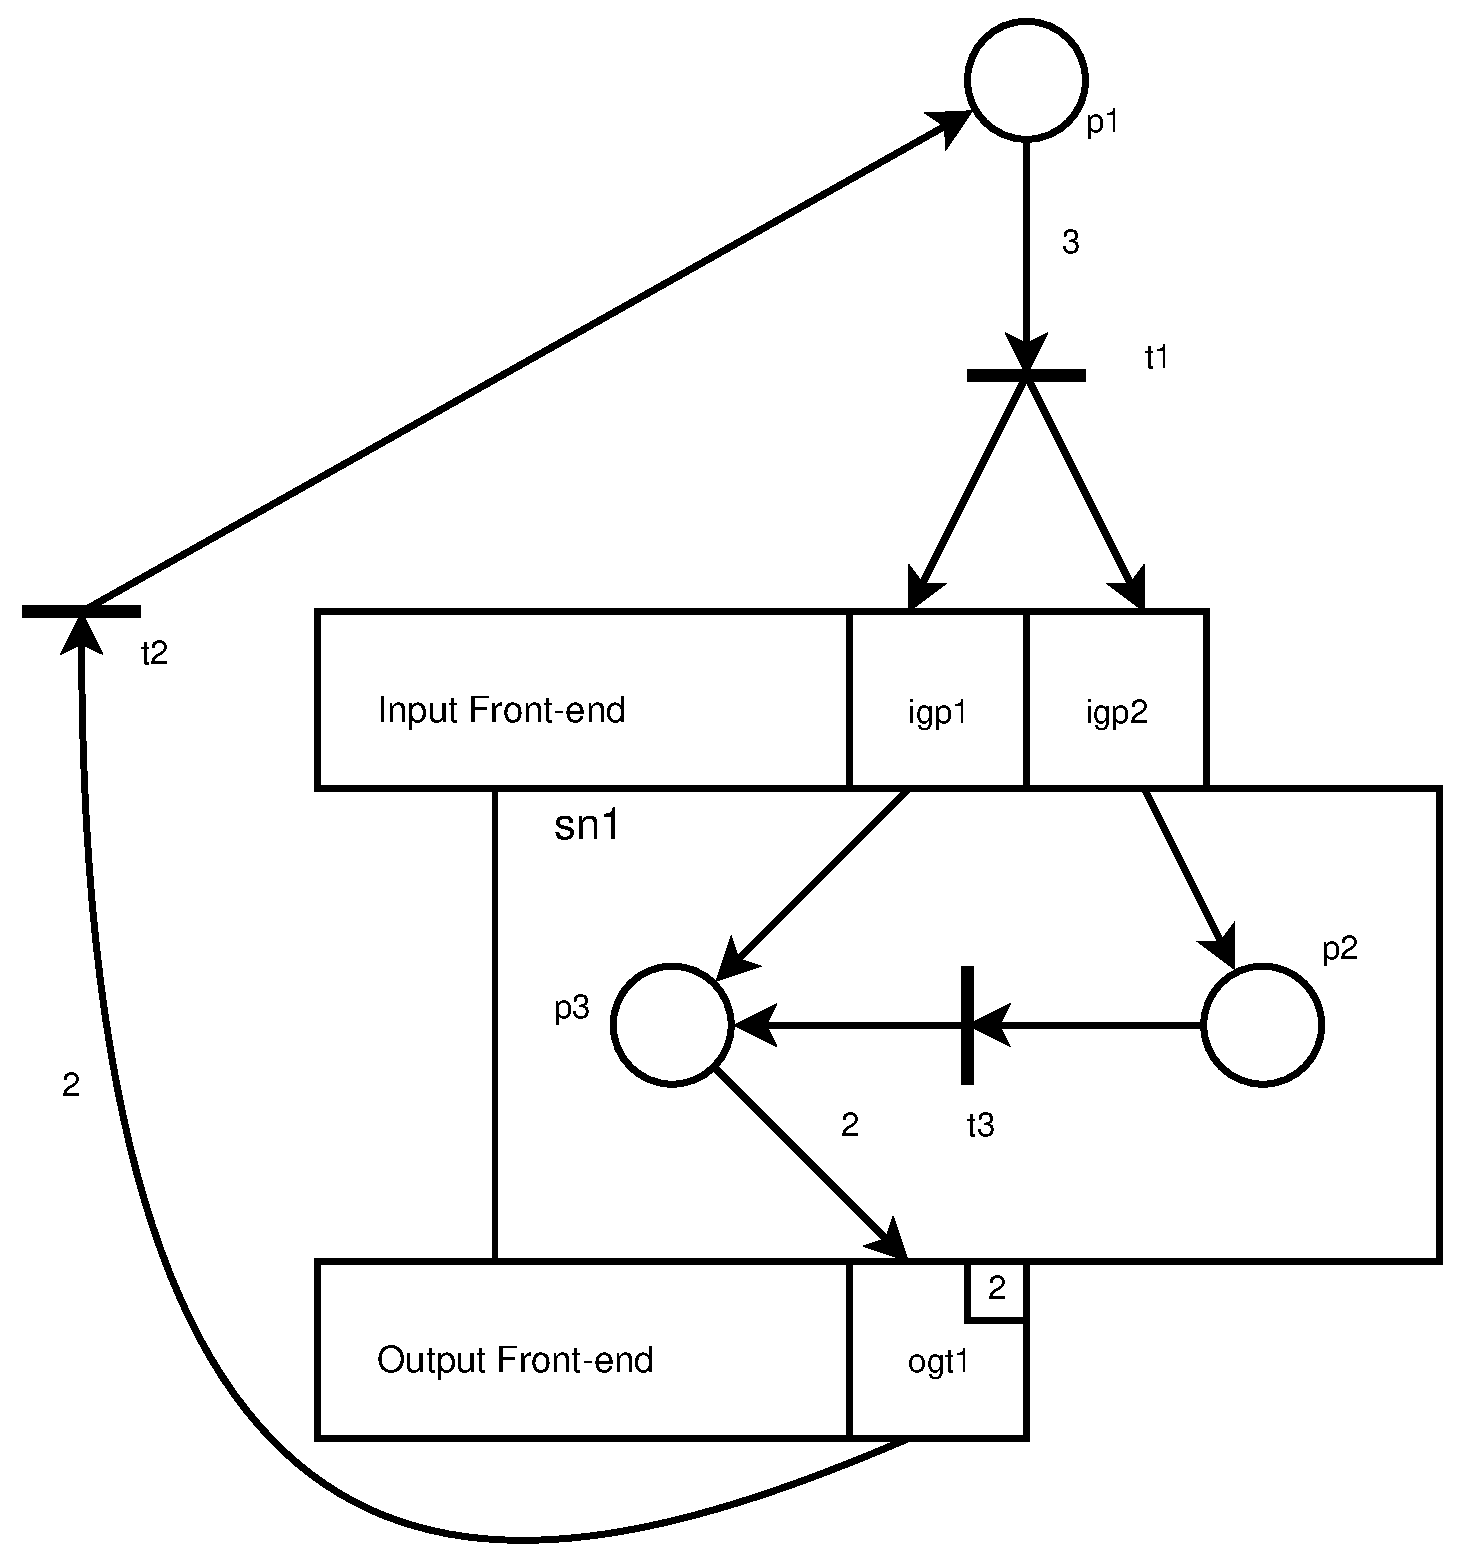
\includegraphics[width=0.60\textwidth]{Figures/PNML-SubredEjemplo1.eps}
\]

...and its PNML representation

\begin{lstlisting}
<subnet id="sn1">
  <interface id="sn1-interface">
    <gate id="igp1" action="input" type="place"/>
    <gate id="igp2" action="input" type="place"/>
    <gate id="ogt1" action="output" type="transition">
      <inscription>
        <text> 2 </text>
      </inscription>
    </gate>
  </interface>
  <content id="sn1-content">
    <place id="p2"/>
    <place id="p3"/>
    <transition id="t3"/>
    <arc id="a2" source="igp2" target="p2"/>
    <arc id="a3" source="igp1" target="p3"/>
    <arc id="a4" source="p3" target="ogt1">
      <inscription>
        <text> 2 </text>
      </inscription>
    </arc>
    <arc id="a5" source="t3" target="p3"/>
    <arc id="a6" source="p2" target="t3"/>
  </content>
</subnet>
<place id="p1"/>
<transition id="t1"/>
<transition id="t2"/>
<arc id="a1" source="p1" target="t1">
  <inscription>
    <text> 3 </text>
  </inscription>
</arc>
<arc id="a2" source="t1" target="igp2"/>
<arc id="a3" source="t1" target="igp1"/>
<arc id="a4" source="ogt1" target="t2">
  <inscription>
    <text> 2 </text>
  </inscription>
</arc>
<arc id="a7" source="t2" target="p1"/>
\end{lstlisting}

The goal is to hide the internal content of the subnet. If we apply XMLEncryption
to the data contained inside the tag \texttt{\textless content\textgreater},\ we will get something like this, depending on the algorithm and key selected for the ciphering.

\begin{lstlisting}
<subnet id="sn1">
  <interface id="sn1-interface">
    <gate id="igp1" action="input" type="place"/>
    <gate id="igp2" action="input" type="place"/>
    <gate id="ogt1" action="output" type="transition">
      <inscription>
        <text> 2 </text>
      </inscription>
    </gate>
  </interface>
  <content id="sn1-content">
    <xenc:EncryptedData xmlns:xenc="http://www.w3.org/2001/04/xmlenc#"  
        Type="http://www.w3.org/2001/04/xmlenc#Element">  
        <xenc:EncryptionMethod  
            Algorithm="http://www.w3.org/2001/04/xmlenc#aes128-cbc"  
            xmlns:xenc="http://www.w3.org/2001/04/xmlenc#" />  
        <xenc:CipherData  
            xmlns:xenc="http://www.w3.org/2001/04/xmlenc#">  
            <xenc:CipherValue  
                xmlns:xenc="http://www.w3.org/2001/04/xmlenc#">  
                  Wr1njyJlYYOM9lAYqcwGCWkw2L4pUjQD2GGVoU9lVZ0wKqHY8y3lGY8FY4i5K
                  3GY8FY4i5K3G8grIe1HRFqe7RtkFiXZgGMeYnQp6oB6ckKp3KFKHVqtucc9rA
                  VzOgC7XAwe61HRFqe6RRVzXjNM9hlVZ0wKqHY8y3l3GY8FY4i5K3G8grIe2xN
                  4u7x7fRtkFiXZgGMeYnQp6oB6ckKp3KFRRVzXjNAtVzOgC7XAw/oe61HRFqe6
                  RRVzXjNMLU5ZgGMeYny8NVPQmUSDX7NRtnR6YnQp6oB6GY8F=
            </xenc:CipherValue>  
        </xenc:CipherData>  
    </xenc:EncryptedData>
  </content>
</subnet>
<place id="p1"/>
<transition id="t1"/>
<transition id="t2"/>
<arc id="a1" source="p1" target="t1">
  <inscription>
    <text> 3 </text>
  </inscription>
</arc>
<arc id="a2" source="t1" target="igp2"/>
<arc id="a3" source="t1" target="igp1"/>
<arc id="a4" source="ogt1" target="t2">
  <inscription>
    <text> 2 </text>
  </inscription>
</arc>
<arc id="a7" source="t2" target="p1"/>
\end{lstlisting} 
 If we try to represent this Petri net we will have the interface of the
 subnet, but the content is a black box.
So it is as follows in the figure:

\begin{figure}[htbp]
\centering
\[
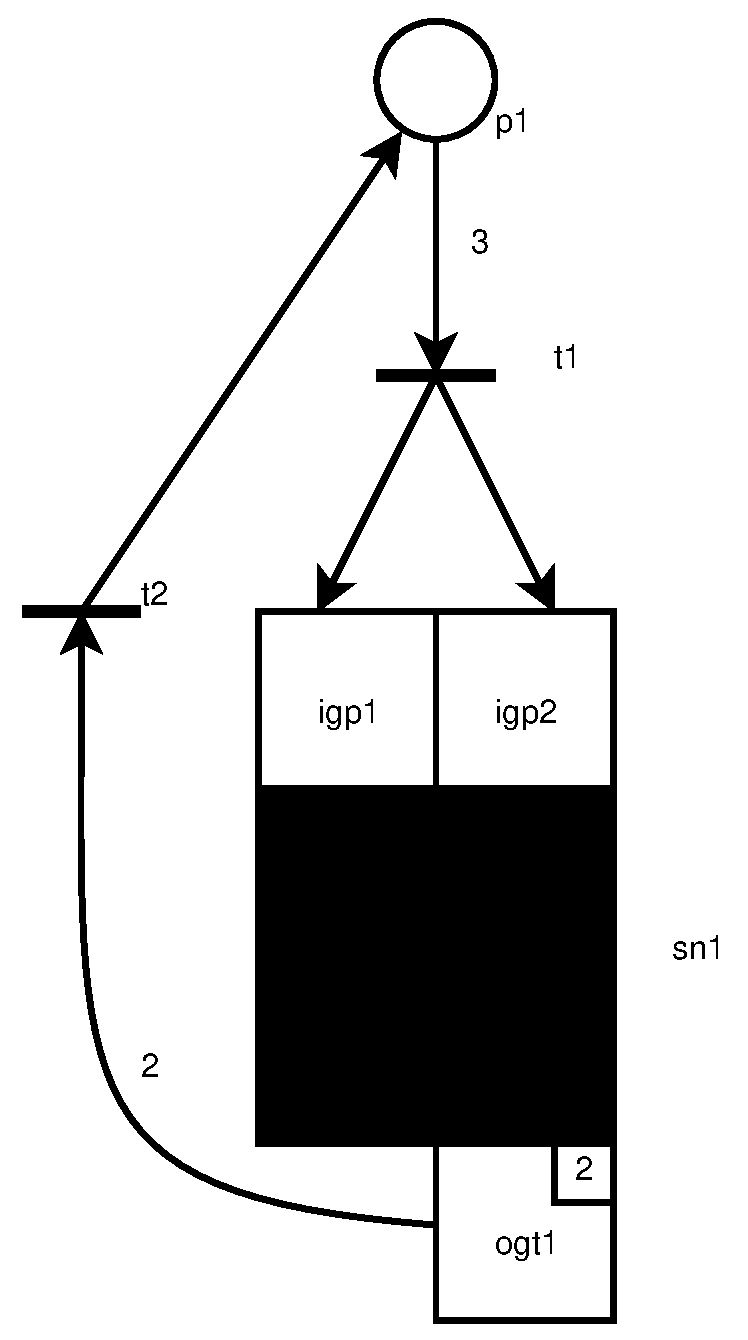
\includegraphics[width=0.40\textwidth]{Figures/XMLENC-SubredEjemplo1.eps}
\]
\rule{35em}{0.5pt}
 \caption{Petri net with hidden subnet}
 \label{fig:XMLENC_SubredEjemplo1} 
\end{figure}

 
\section{Examples}

\subsection{Hidding several subnets}\label{Example several subnets}

One important thing is that I can cipher several subnets of the same Petri
net with distinct options. For example, if there are two subnets for both
two distinct receivers each one of the subnets can be configured in order
to each subnet can be decrypted by its own receiver.

//TODO

\subsection{Critical processes}

//TODO

\section{Conclusions}

As we have seen, one of the applications of subneting Petri nets and represent
them in PNML is that I can apply standard processes based on XML. In this
case, once defined and represented a subnet in PNML, I have apply XMLEncryption in order to hide the internal structure of the subnet.

Actually, there are several options to apply XMLEncryption, such as the algorithm
or the key. The exact election of those option values is responsibility of the Petri net sender. For example:
\begin{itemize}
 \item Maybe both parts (sender and receiver) have a common
set of keys, so they can use it in order to encrypt and decrypt the subnet.
 \item Other common use is that
the key is defined inside the options but it is ciphered itself. If the receiver
have a pair of keys (public and private) and an asymmetrical algorithm (such as Diffie-Hellman or RSA) , the symmetric key can be ciphered by
the sender with the receiver's public key. In this case, only the receiver
can decrypt it using his private key.
\end{itemize}
Other important thing is that several subnets in the same net can be encrypted with different
options. This is used, for example, for  one receiver
to decrypt the subnet addressed to him but no other one.

With the explained in this chapter, the privacy of parts of a Petri net is guarantied.    
